\documentclass{article}
\usepackage{tikz, comment}
\usepackage{pifont}
\usepackage{fontspec, pgfplots}
\usetikzlibrary{arrows, decorations.markings, decorations.pathreplacing}
\begin{comment}
:Title: Not defined yet
:Tags: adjugate, classical adjoint;end behavior;additive inverse of a matrix;nth partial sum;perimeter
:Prob: 0.3175;0.2746;0.2583;0.2562;0.252
:Author: Prof.Hu Ji-shan, HKUST
:Slug: No name yet

Description Here.........
\end{comment}
\begin{document}\centering 

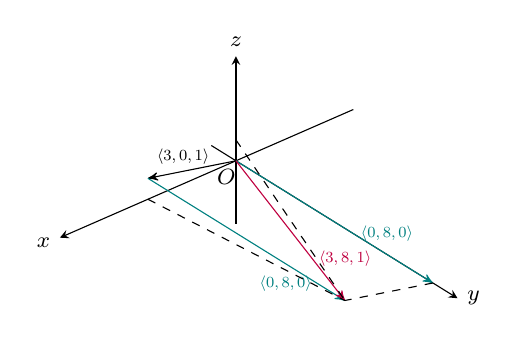
\begin{tikzpicture}[font=\footnotesize]
\pgfplotsset{compat=1.8}

\begin{axis}
[z post scale=1, axis lines = center, view={140}{50}, ticks=none, 
axis background, xlabel = {$x$}, ylabel ={$y$}, zlabel ={$z$}, domain =0:1, y domain =0:1,
xmin =-4.0,
xmax =6.0,
ymin =-1.0,
ymax =9,
zmin =-3, 
zmax =5,
samples =10, samples y =40, z buffer =sort,
every axis x label/.style={
    at={(ticklabel* cs:1)},
    anchor= east, yshift =-2
},
every axis y label/.style={
    at={(ticklabel* cs:1)},
    anchor= west,
},
every axis z label/.style={
    at={(ticklabel* cs:1)},
    anchor= south
}]

\node[xshift=4, yshift=4, label={-100:{$O$}}] at (axis cs:0,0,0) {};

\addplot3[->, >=stealth'] coordinates
        {(0,0,0) (3,0,1)}node[above, midway, pos=0.6, xshift=0, yshift=0, scale=0.7]{$\langle 3,0,1 \rangle$};

\addplot3[teal, ->, >=stealth'] coordinates
        {(0,0,0) (0,8,0)}node[right, midway, pos=0.6, xshift=0, yshift=0, scale=0.7]{$\langle 0,8,0 \rangle$};

\addplot3[teal, ->, >=stealth'] coordinates
        {(3,0,1) (3,8,1)}node[below, midway, pos=0.7, xshift=0, yshift=-2, scale=0.7]{$\langle 0,8,0 \rangle$};

\addplot3[purple, ->, >=stealth'] coordinates
        {(0,0,0) (3,8,1)}node[right, midway, pos=0.7, xshift=0, yshift=0, scale=0.7]{$\langle 3,8,1 \rangle$};
        
\addplot3[dashed] coordinates
        {(3,8,1) (3,0,0)};
        
\addplot3[dashed] coordinates
        {(3,8,1) (0,8,0)};

\addplot3[dashed] coordinates
        {(3,8,1) (0,0,1)};

\end{axis}

\end{tikzpicture}
\end{document}